\documentclass[a4paper,9pt]{article}

\usepackage[margin=1.5cm]{geometry}
\usepackage{graphicx}
\usepackage{amsmath}
\usepackage{booktabs}
\usepackage{float}
\usepackage{enumitem}
\usepackage{titlesec}

\setlength{\parindent}{0pt}
\setlength{\parskip}{3pt}
\setlist{nosep,leftmargin=*}
\titlespacing*{\section}{0pt}{6pt}{3pt}

\title{\vspace{-1cm}\textbf{Assignment 1: Offensive Language Classification}}
\author{Syed Hassan Imam Naqvi}
\date{}

\begin{document}
\maketitle
\vspace{-1cm}

\section{Introduction}

The aim of this assignment was to classify tweets as
\textit{offensive} or \textit{nonoffensive}. I used Naive Bayes and
Logistic Regression and checked their performance with accuracy and
F1-score. The dataset had 12,896 training tweets and 3,250 test tweets.

\section{Naive Bayes and Smoothing}

I implemented Multinomial Naive Bayes using word counts. I used
additive smoothing to avoid zero probabilities:

\[
P(w \mid c) =
\frac{\text{count}(w,c)+k}
{\text{total}(c)+k|V|}
\]

Here, \(k\) is the smoothing value and \(|V|\) is the number of words
in the vocabulary. Unknown words in test tweets are ignored. I also
used log probabilities for classification.

I tested different values of \(k\). The results are shown below.

\begin{table}[H]
\centering
\small
\begin{tabular}{ccc}
\toprule
\textbf{Smoothing k} & \textbf{Accuracy} & \textbf{F1-score} \\
\midrule
0.01 & 82.40\% & 49.38\% \\
0.1  & 84.03\% & 52.95\% \\
0.5  & 85.29\% & 53.86\% \\
1.0  & 85.72\% & 51.57\% \\
2.0  & 86.03\% & 47.21\% \\
5.0  & 84.80\% & 33.24\% \\
10.0 & 83.57\% & 20.06\% \\
\bottomrule
\end{tabular}
\caption{Naive Bayes results for different smoothing values.}
\end{table}

\begin{figure}[H]
\centering
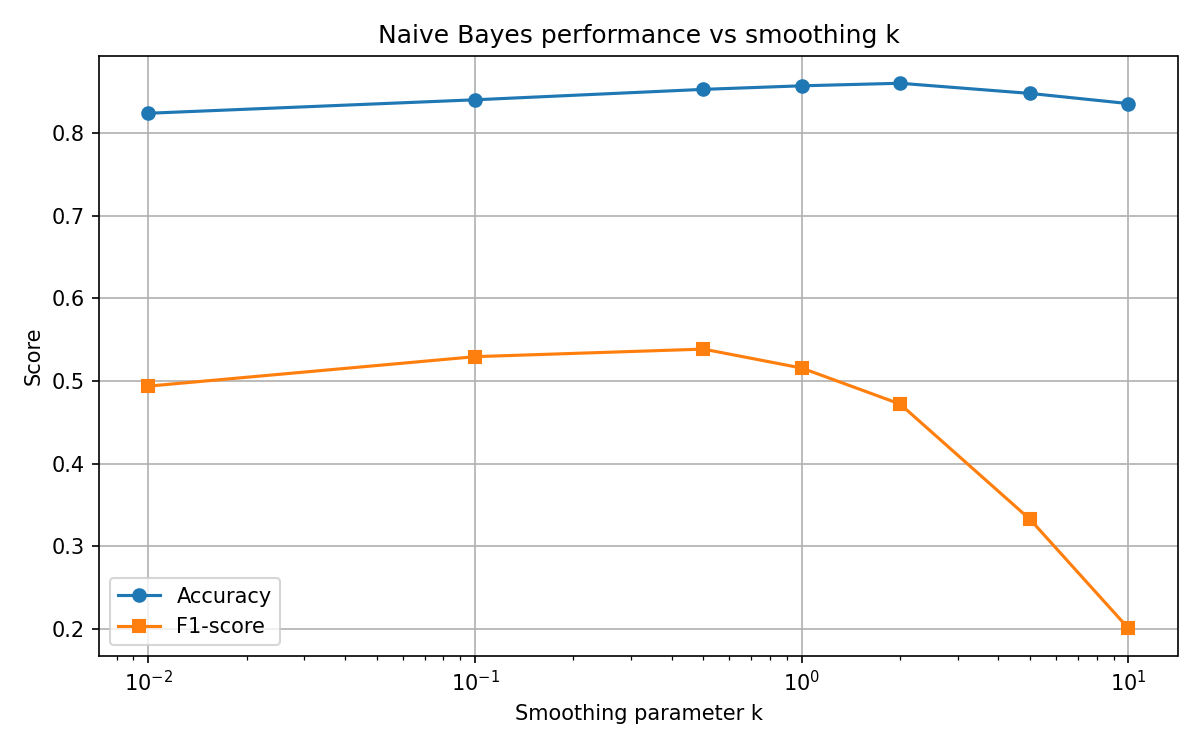
\includegraphics[width=0.58\linewidth]{smoothing_k_plot.png}
\caption{Accuracy and F1-score for different smoothing values.}
\end{figure}

When \(k\) is very small, a word that appears in only one class gets
almost zero probability in the other class. Rare words can then have
too much effect, and the model may fit the training data too closely.
When \(k\) is large, word counts matter less and words get more similar
probabilities in each class. A small increase in \(k\) first improves
the results, but very large values make performance worse. The best
F1-score was 53.86\% at \(k=0.5\). The highest accuracy was 86.03\%
at \(k=2.0\).

\section{Feature Engineering}

I tested two more feature sets with Naive Bayes:

\begin{itemize}
    \item \textbf{Feature set 1 : Stopword removal and lowercasing:}
    I removed common words and changed all words to lowercase. This
    joins words that are written with different capital letters.

    \item \textbf{Feature set 2 : Unigrams and bigrams:}
    I used single words and pairs of words next to each other.
    Bigrams can help the model learn short phrases.
\end{itemize}

\begin{table}[H]
\centering
\small
\begin{tabular}{lcc}
\toprule
\textbf{Feature set} & \textbf{Accuracy} & \textbf{F1-score} \\
\midrule
Baseline bag-of-words & 85.72\% & 51.57\% \\
Stopword removal and lowercasing & 83.91\% & 51.71\% \\
Unigrams and bigrams & 86.06\% & 50.71\% \\
\bottomrule
\end{tabular}
\caption{Comparison of Naive Bayes feature sets.}
\end{table}

Bigrams gave the highest accuracy, but their F1-score was lower than
the baseline. Stopword removal gave a slightly higher F1-score but
lower accuracy. So, neither feature set improved both scores.

\section{Logistic Regression}

I also implemented Logistic Regression using a bag-of-words
representation. The feature matrix had 25,889 features. I trained the
model for 10 epochs using mini-batch gradient descent, a learning rate
of 0.01 and regularization parameter \(C=0.1\).

The features are binary: a feature is 1 if a word appears in a tweet
and 0 if it does not. The loss is added over each batch of 100 tweets.
When I used the average loss for each batch instead, \(C=0.1\) was too
strong and the model almost always predicted nonoffensive.

The model achieved 83.51\% accuracy and 51.71\% F1-score.

\section{Overall Results and Discussion}

\begin{table}[H]
\centering
\small
\begin{tabular}{lcc}
\toprule
\textbf{Model} & \textbf{Accuracy} & \textbf{F1-score} \\
\midrule
Naive Bayes (\(k=1\)) & 85.72\% & 51.57\% \\
Logistic Regression & 83.51\% & 51.71\% \\
\bottomrule
\end{tabular}
\caption{Comparison of the two baseline models.}
\end{table}

About 82\% of the test tweets are nonoffensive. A model that always
predicts nonoffensive would already get about 0.819 accuracy. This is
why I also look at the F1-score for the offensive class.

Naive Bayes had higher accuracy, while Logistic Regression had a
slightly higher F1-score. The F1-scores were very close. This shows
why it is useful to check both accuracy and F1-score.

\section{Bonus Discussion Questions}

\textbf{Question 1: What is the effect of \(k\) on word probabilities?}

The value \(k\) is added to every word count, so no word gets a
probability of zero. If \(k\) is much larger than the word counts,
words get almost the same probability in each class. The model then
depends more on how common each class is.

\textbf{Question 2: Does shuffling the order of words in a document
affect Naive Bayes results?}

No. Naive Bayes counts words but does not look at their order.
Shuffling the words does not change the word counts, so the results
stay the same.

\textbf{Question 3: Why do we use Softmax if the model already gives
a score for each class?}

Softmax changes the scores into probabilities between 0 and 1.
These probabilities add up to 1, so we can compare the classes and
choose the one with the higher probability.

\textbf{Question 4: How many times do we need to train to find the
best threshold?}

Only once. We train the model, then use its predictions on a
validation set to choose the threshold that gives the best score.
We do not need to train the model again for each threshold.

\vspace{2pt}
\textbf{Git commit hash:} \textit{Add your actual commit hash here if you complete the Git bonus.}

\end{document}



